\begin{figure}
  \centering
  \captionsetup{justification=centering}
  \begin{subfigure}[b]{0.4\linewidth}
    \label{subfig:top_view}
    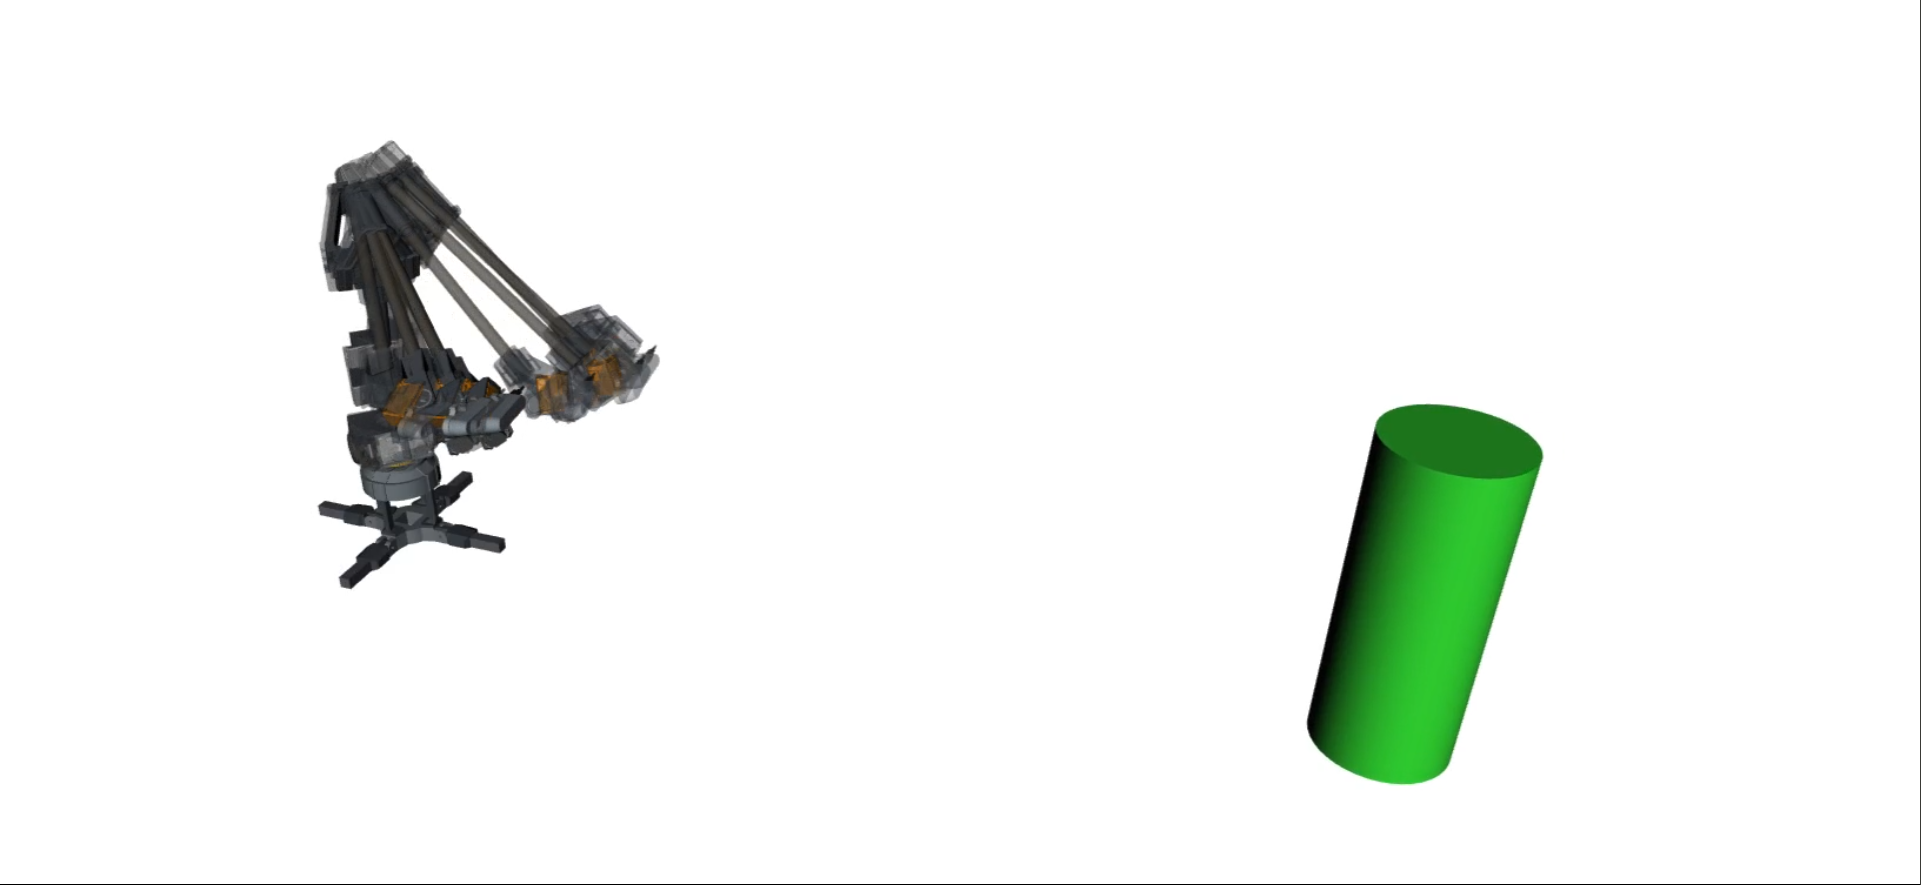
\includegraphics[width=\linewidth]{avoiding_moving_obs_1.png}
     \caption{}
  \end{subfigure}
  \begin{subfigure}[b]{0.4\linewidth}
    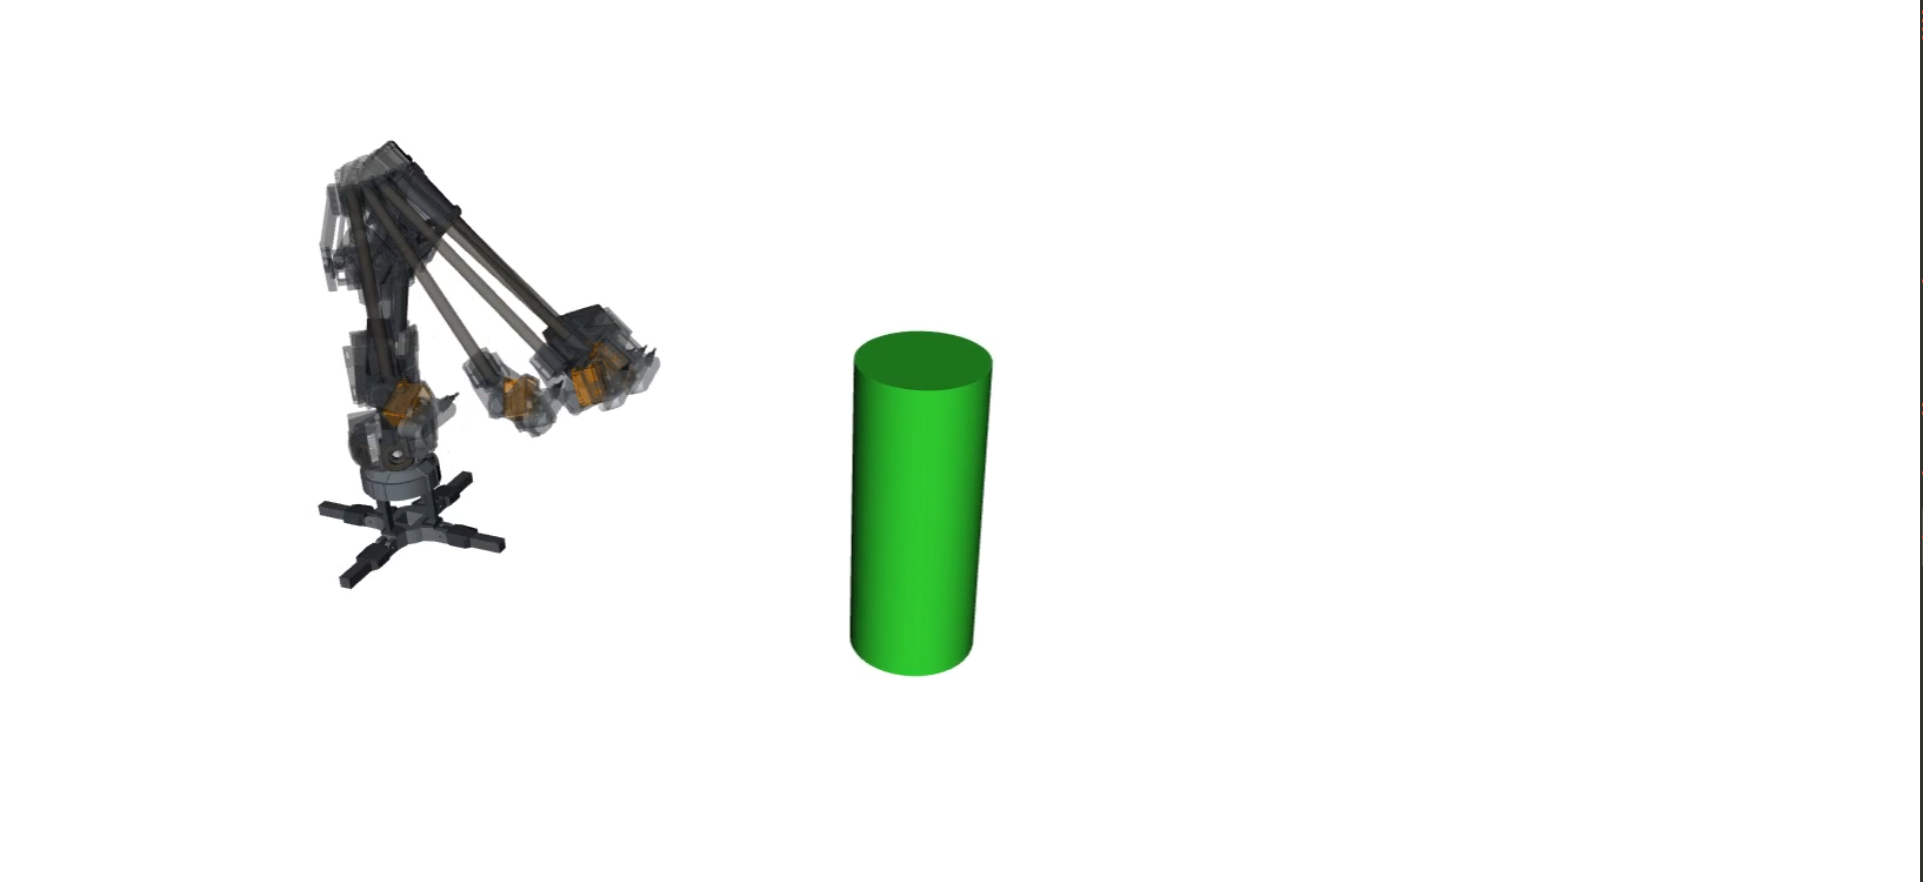
\includegraphics[width=\linewidth]{avoiding_moving_obs_2.png}
    \caption{}
  \end{subfigure}
  \begin{subfigure}[b]{0.4\linewidth}
    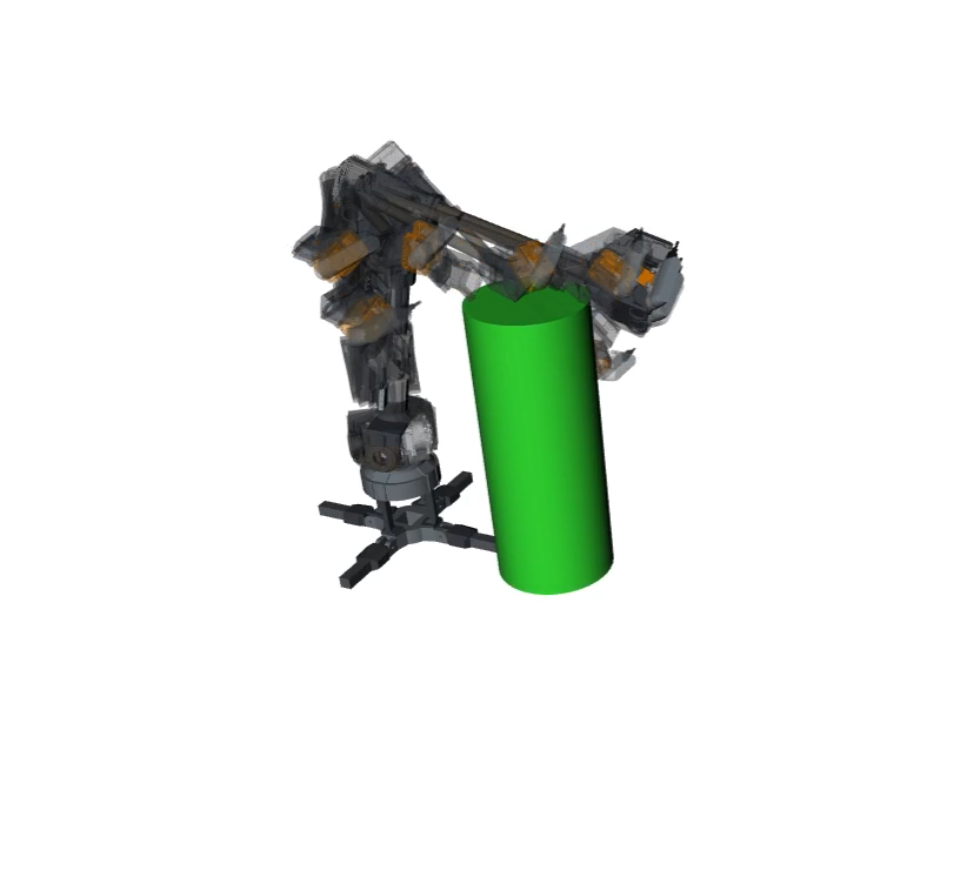
\includegraphics[width=\linewidth]{avoiding_moving_obs_3.png}
    \caption{}
  \end{subfigure}
  \begin{subfigure}[b]{0.4\linewidth}
    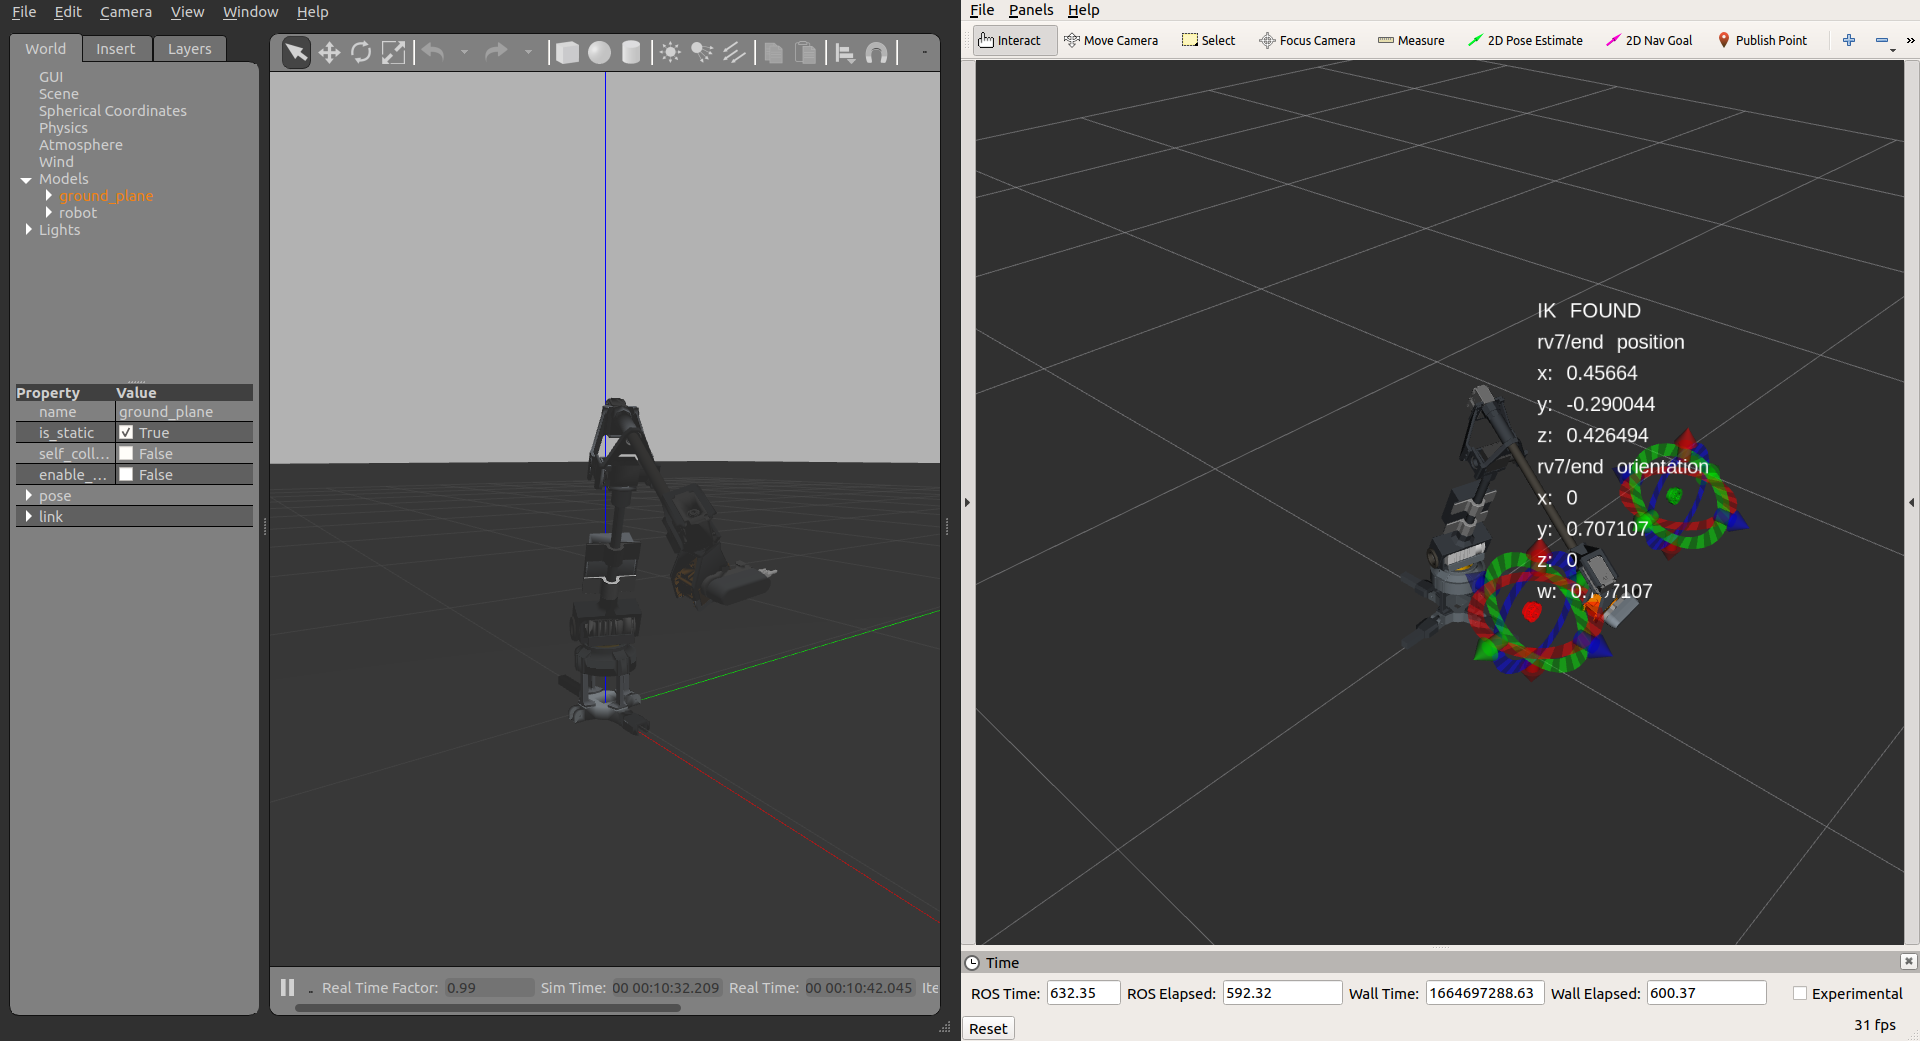
\includegraphics[width=\linewidth]{avoiding_moving_obs_gazebo.png}
    \caption{}
  \end{subfigure}

  \caption{The chronology of attempts at avoiding a moving obstacle
  when the obstacle approaches the robot. The planning algorithm fails at
  avoiding the cylinder before it passes the $x-location$ of the poses, $c_{intial}$
  and $c_{goal}$. (c) shows the planner successfully provide 
  a non-colliding solution when the cylinder is moving away from robot. (d) shows the Gazebo as 
  the physic engine to replicate the robot hardware and encoders feedback and
  the cyclical space initialization.}
  \label{fig:avoiding_moving_obs}
\end{figure}
